\section*{Spielen mit Schießpulver: \\
The Powder Toy}
\hypertarget{powdertoy}{}
\label{powdertoy}
\NewsAuthor{Horst JENS}

\textbf{Dieser Artikel beschreibt das Physik/Chemie-Simulationsspiel \textit{The Powder Toy [1]} und zeigt einen kleinen Teil der Möglichkeiten die man damit anstellen kann. \textit{The Powder Toy} ist freie (free/libre Open Source) Software, die von jedem Interessierten benutzt, kopiert, verändert und weiterentwickelt werden kann, gemäß den vier Grundfreiheiten welche die \textit{GPL-Lizenz [2]} gewährt.}

\begin{center}
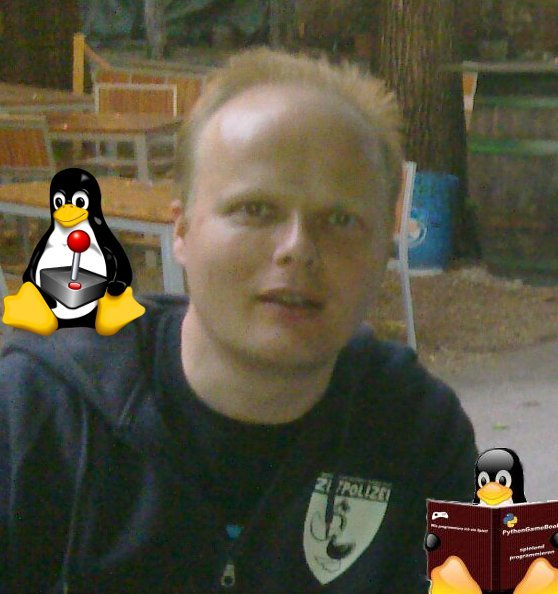
\includegraphics[width=4cm]{horst2011mitdoppeltux.jpg} \\
\footnotesize{Horst JENS. Bildrechte: [3], cc-by-sa}
\end{center}


{Hinweis:} Wenn Sie Internetverbindung haben, schauen Sie sich die folgenden Bilder online an in Farbe oder drucken Sie diesen Artikel auf einem Farbdrucker aus.

\subsection*{erst die Arbeit...}

Auf der Homepage von \textit{The Powder Toy [1]} kann man sich die aktuelle Version oder die noch in Entwicklung befindliche, allerneuste Beta-Version für verschiedene Betriebssysteme downloaden. Zum nur damit spielen ist nichts weiter notwendig (Download starten und Spiel installieren). Weil ich mir den \textbf{Sourcecode} genauer anschauen will habe ich mir das Programm selbst \textbf{kompiliert}. Dazu muss ich mir die tagesaktuelle Version des Programms von Github herunterladen. Wie das geht beschreibt das englische Tutorial \href{http://goo.gl/LK4z01}{\textit{Compile for Linux [4]}} im The Powder Toy Wiki ganz gut. Für Windows und Mac User gibt es im Wiki eigene Tutorials. Hier sind die Schritte die ich gemacht habe (Ubuntu Linux, 64-bit, 2 Prozessoren):

\begin{itemize}
\item Ein Terminal öffnen (Alt+STR+T) und folgendes eintippen 
\begin{center}
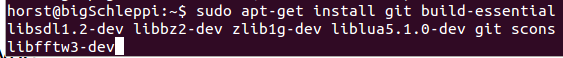
\includegraphics[width=\linewidth]{powdertoy/zeile1.png}
\end{center}
\item In jenes Verzeichnis wechseln unter welchem The Powder Toy installiert werden soll. Nachdem ich mir ein \textit{games} Verzeichnis erstellt hatte (\texttt{mkdir games}) war das bei mir das Verzeichnis \texttt{home/horst/games} deshalb musste ich dorthin wechseln mit: \texttt{cd games}  
\item Jetzt die neues Version von Github klonen (folgenden Befehl in eine einzige Zeile schreiben):
\begin{center}
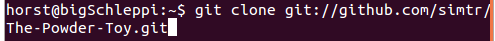
\includegraphics[width=\linewidth]{powdertoy/zeile2.png}
\end{center}
\item das Kommando \texttt{ls} (oder ein Blick auf meinen Datei-Manager) verrät mir dass ich ein neues Verzeichnis auf meiner Festplatte habe, in welches ich gleich hineinwechsle: \texttt{cd The-Powder-Game}
\item Jetzt kann der Kompiliervorgang starten! Ich tippe:
\begin{center}
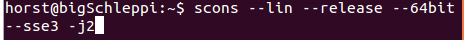
\includegraphics[width=\linewidth]{powdertoy/zeile3.png}
\end{center} Was die Parameter bedeuten wird im Wiki erklärt. Wer kein 64bit System hat lässt das \texttt{--64bit} weg, wer einen alten Computer hat lässt das \texttt{--sse3} weg und wer 4 Prozessoren hat schreibt \texttt{-j4} anstatt so wie ich \texttt{-j2} oder lässt diesen Parameter ganz weg. Nach ein paar Minuten ist das Programm fertig compiliert und befindet sich im Unterverzeichnis 'build'
\item In dieses Unterverzeichnis hineinwechseln, entweder per Dateimangaer oder per \texttt{cd build} und \texttt{ls}.
\item Je nachdem welche Parameter man gewählt hat heisst das Programm jetzt unterschiedlich. Meines heisst \texttt{powder64} und ich kann es per Doppelklick starten oder per \texttt{.\\powder64}.
\end{itemize}
% from master file
\end{multicols}
\SepRule
%\newpage
\begin{multicols}{2}
% from powdertoypictures
\subsection*{...dann das Vergnügen}

The Powder Toy begrüßt den Spieler äußerst unspektakulär:
\begin{center}
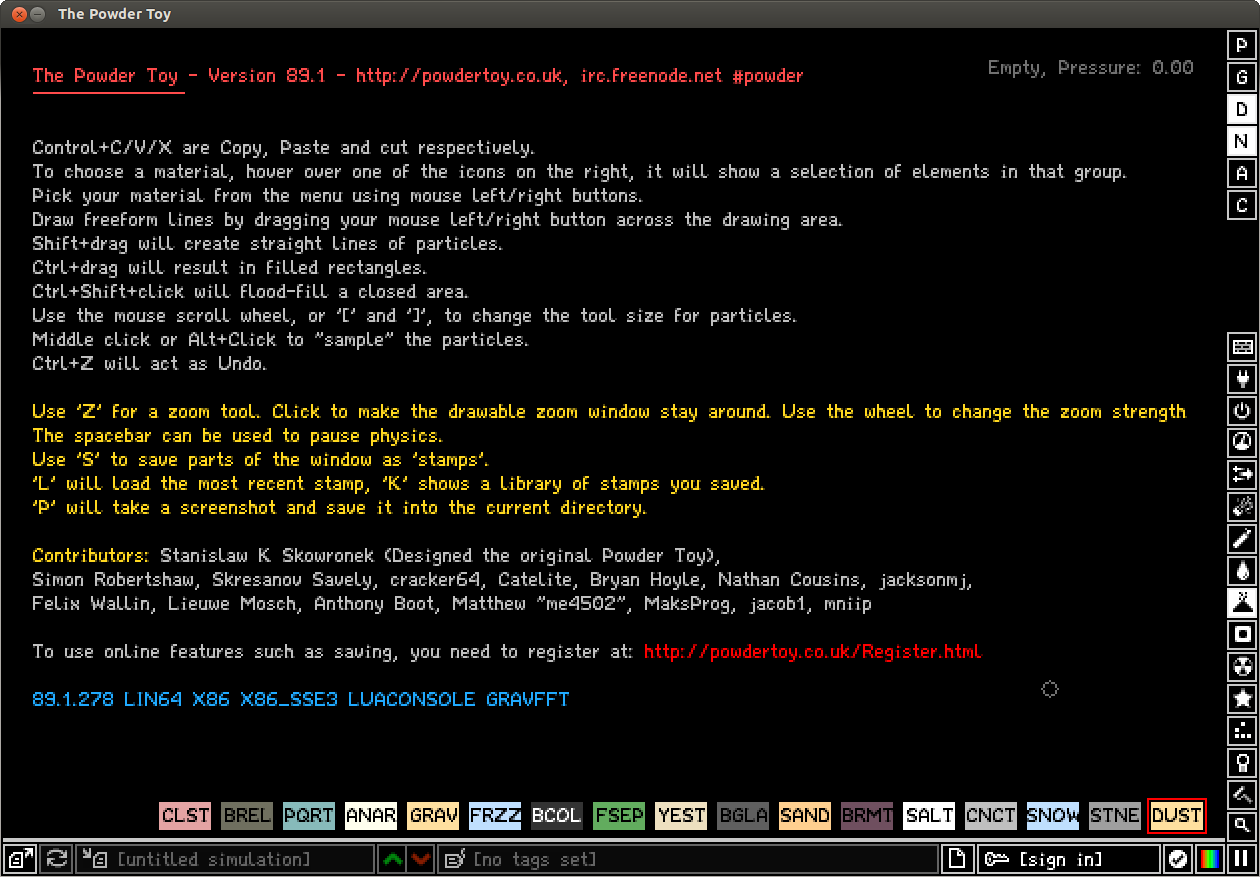
\includegraphics[width=\linewidth]{powdertoy/powdertoy-intro.png}
\end{center}

Das wichtigste Icon ist jenes mit dem man die Fenstergröße einstellen kann bzw. den Fullscreen-Modus aktiviert. Es ist das 3. Icon von rechts auf der Iconleiste am unteren Bildschirmrand, ein weisser Kreis mit einem Haken drin. Dieses Icon anklicken und entweder auf 'Large Screen' oder 'Full Screen' klicken, zumindest wenn man einen großen Monitor besitzt. 

Jetzt kann es losgehen, zum Aufwärmen zerstöre ich einen Unterwasserbunker mittels Sprengstoff:
Mit der 'Open' Schaltfläche ganz links unten öffne ich (sofern Internetverbindung vorhanden ist) eine hübsche Vorlage:
\begin{center}
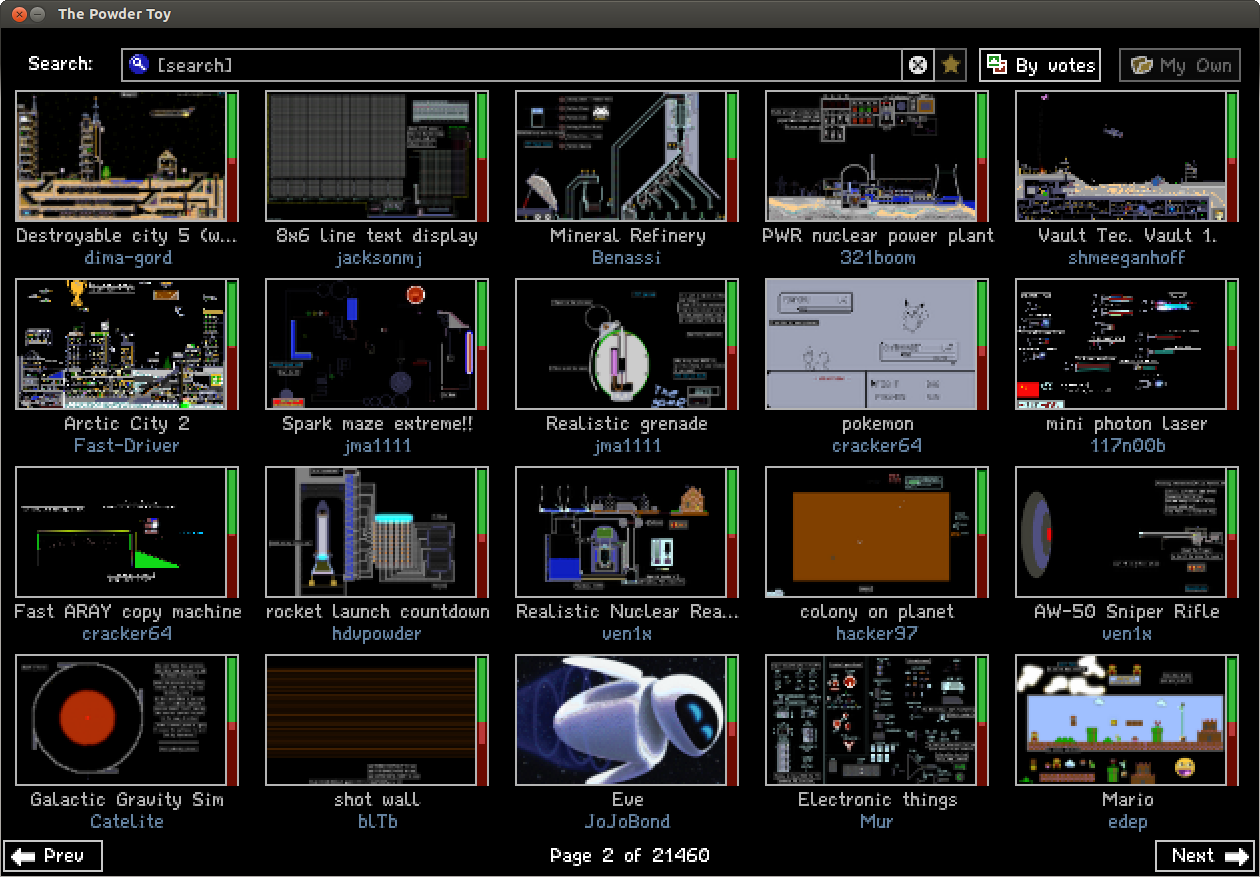
\includegraphics[width=\linewidth]{powdertoy/powdertoy-auswahl.png}
\end{center}

In diesem Fall den 'Underwater bunker' aber eigentlich ist es nicht so wichtig welche Szene ich öffne.
\begin{center}
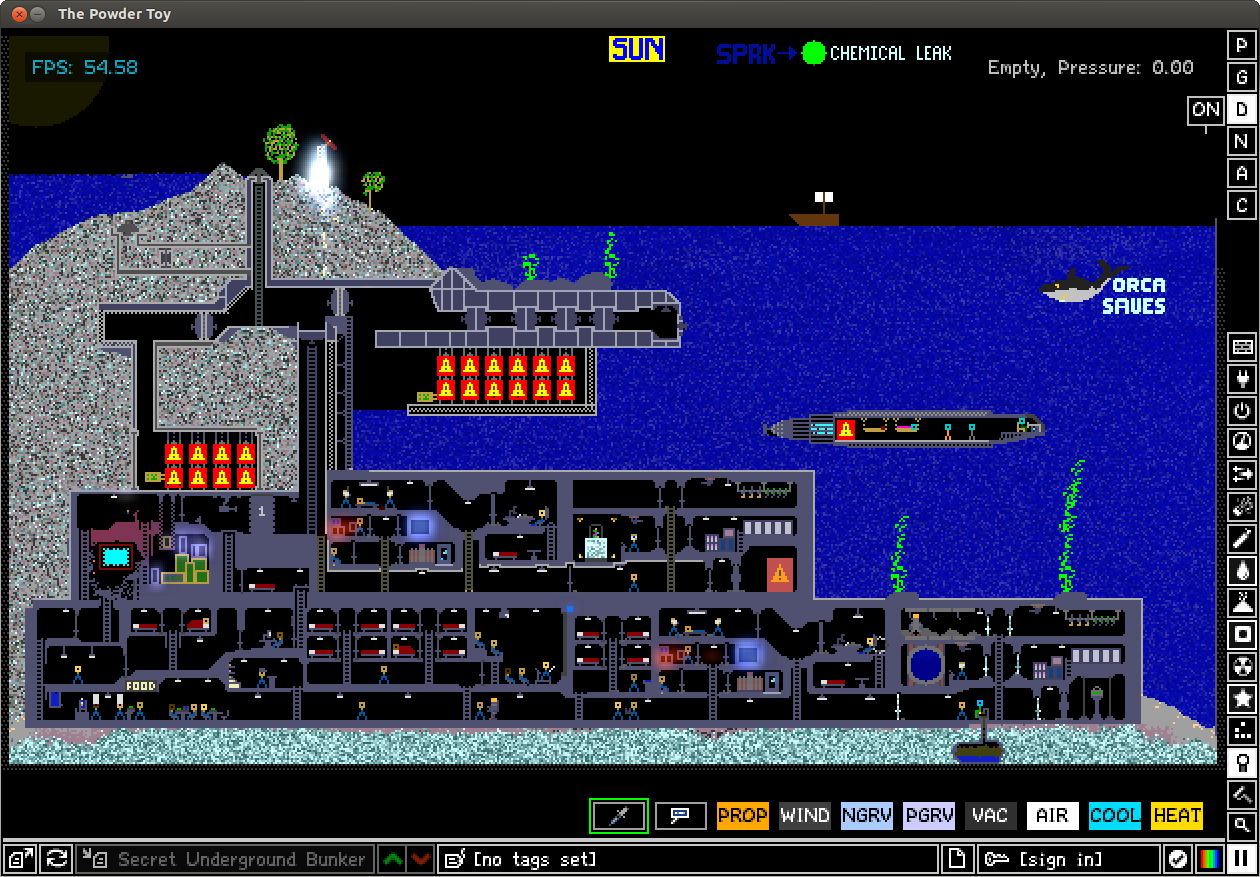
\includegraphics[width=\linewidth]{powdertoy/powdertoy-bu1.png}
\end{center}
Man beachte die hohe \textit{Framerate} links oben von fast 60 \textit{FPS} und das sich das Spiel im Pause-Modus befindet. Mit dem Pause-Icon (ganz rechts unten im Eck) kann ich jederzeit zwischen Pause und Echtzeit umschalten.

Die Spielszene empfiehlt (Schrift oben im Bild) mittels eines Funken (Sprk) das 'Gift-Leck' (Poison-Leak) anzuzünden, aber ich habe andere Plände:

Ich klicke das Menü für Explosionsstoffe rechts an und wähle bei der Auswahl unten \href{https://de.wikipedia.org/wiki/Thermit}{Thermit} (im Spiel als 'THRM' bezeichnet), welches laut Spielbeschreibung sehr heiss verbrennt und laut Wikipedia sehr gut geeignet ist um Wolkenkratzer und Stahlkonstruktionen abzureißen. (Ich hätte auch mit dem Luben-Icon (2. von unten, Iconleiste rechts) nach allen Verfügbaren Stoffen suchen können). Noch im Pause-Modus male ich wie mit einem Malprogramm die beiden Bunkerräume unter dem 2. Baum von links voll mit Thermit.
\begin{center}
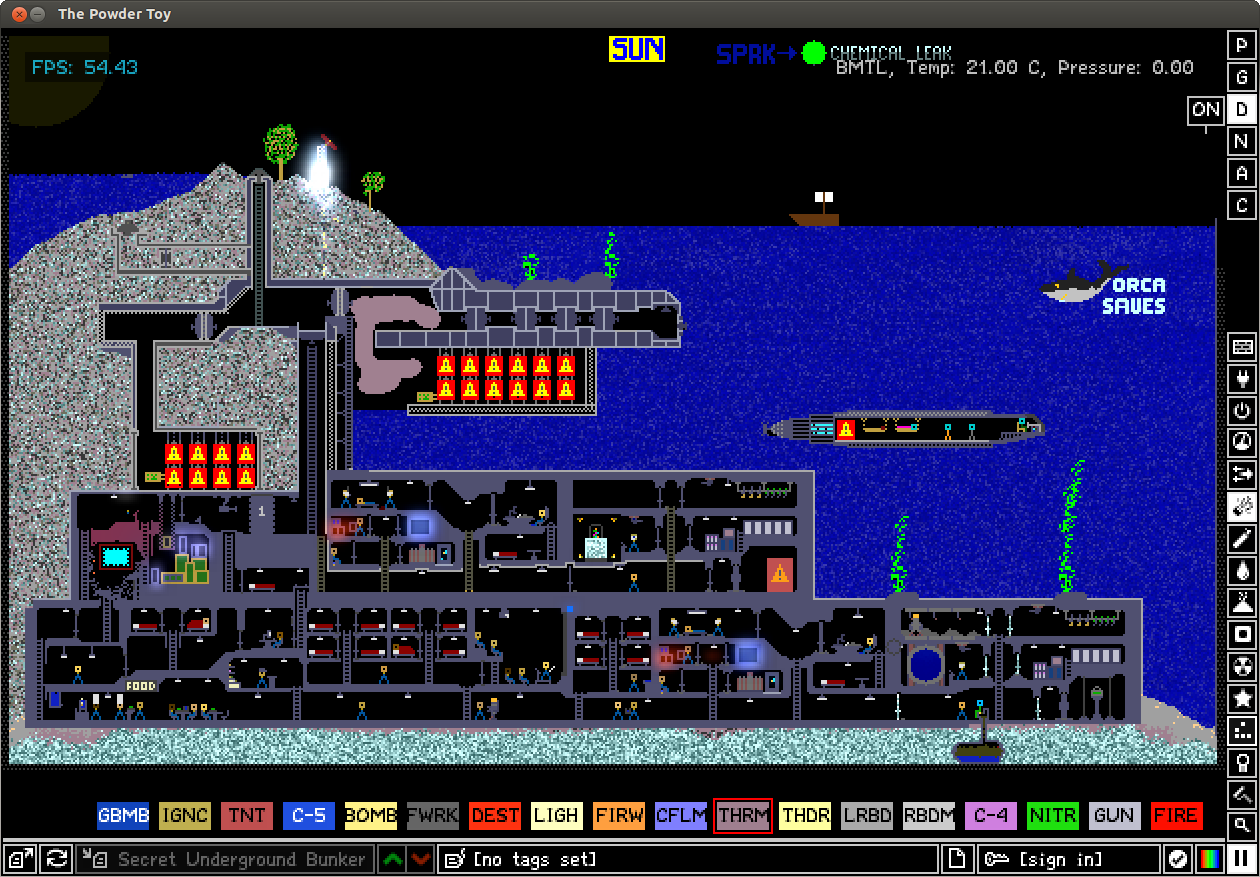
\includegraphics[width=\linewidth]{powdertoy/powdertoy-bu2.png}
\end{center}
Nach Umschalten auf den Echtzeit - Modus (Icon ganz rechts unten) merke ich dass mein Thermit nicht nur nach unten rieselt sondern durch eine Taucherluke auch gleich ins Wasser. Normalerweise verhindert die Luftblase über der Taucherluke das Eindringen von Wasser in den Bunker, aber da ich die Luft mit Thermit ersetzt habe und das mein herunter-rieselnder Sprengstoff Wasser verdrängt (Die Physik in The Powder Game ist etwas vereinfacht) schwappt jetzt üblelriechendes Meerwasser zu in meinen Bunker. Womöglich rosten dadurch die Giftmüllfässer ! 

Schnell klicke ich unten rechts auf 'Fire' und klicke damit (im Echtzeitmodus) auf das Thermit, um das Wasser per Hitze zu vertreiben.
\begin{center}
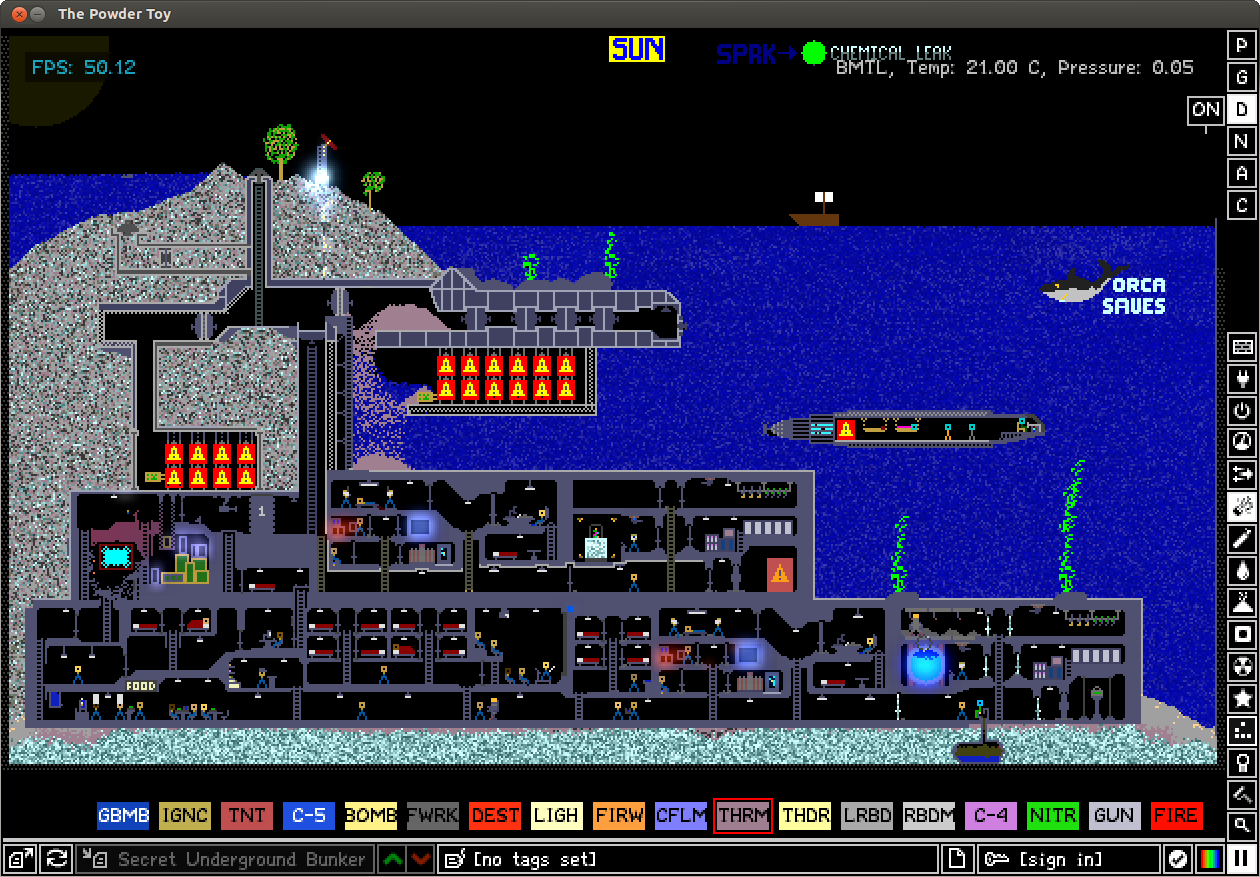
\includegraphics[width=\linewidth]{powdertoy/powdertoy-bu3.png}
\end{center}

Zu dumm aber auch, ich habe das herunterrieselnde Thermit angezündet, nicht das neben den Giftfässern:
\begin{center}
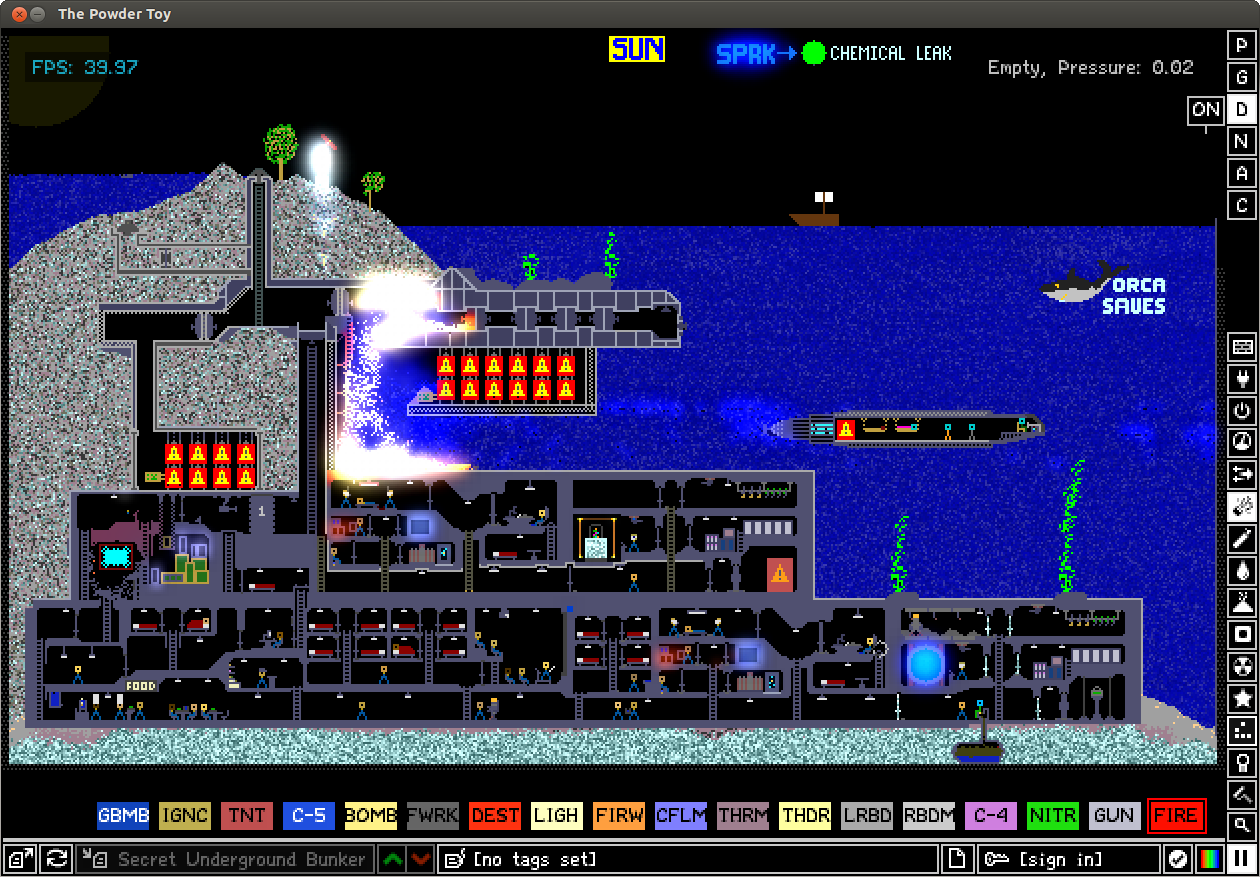
\includegraphics[width=\linewidth]{powdertoy/powdertoy-bu4.png}
\end{center}

Oha, das Feuer frisst sich nach oben in den Berg und nach unten in den Bunker!. Wenigstens lässt es die Giftfässer in Ruhe
\begin{center}
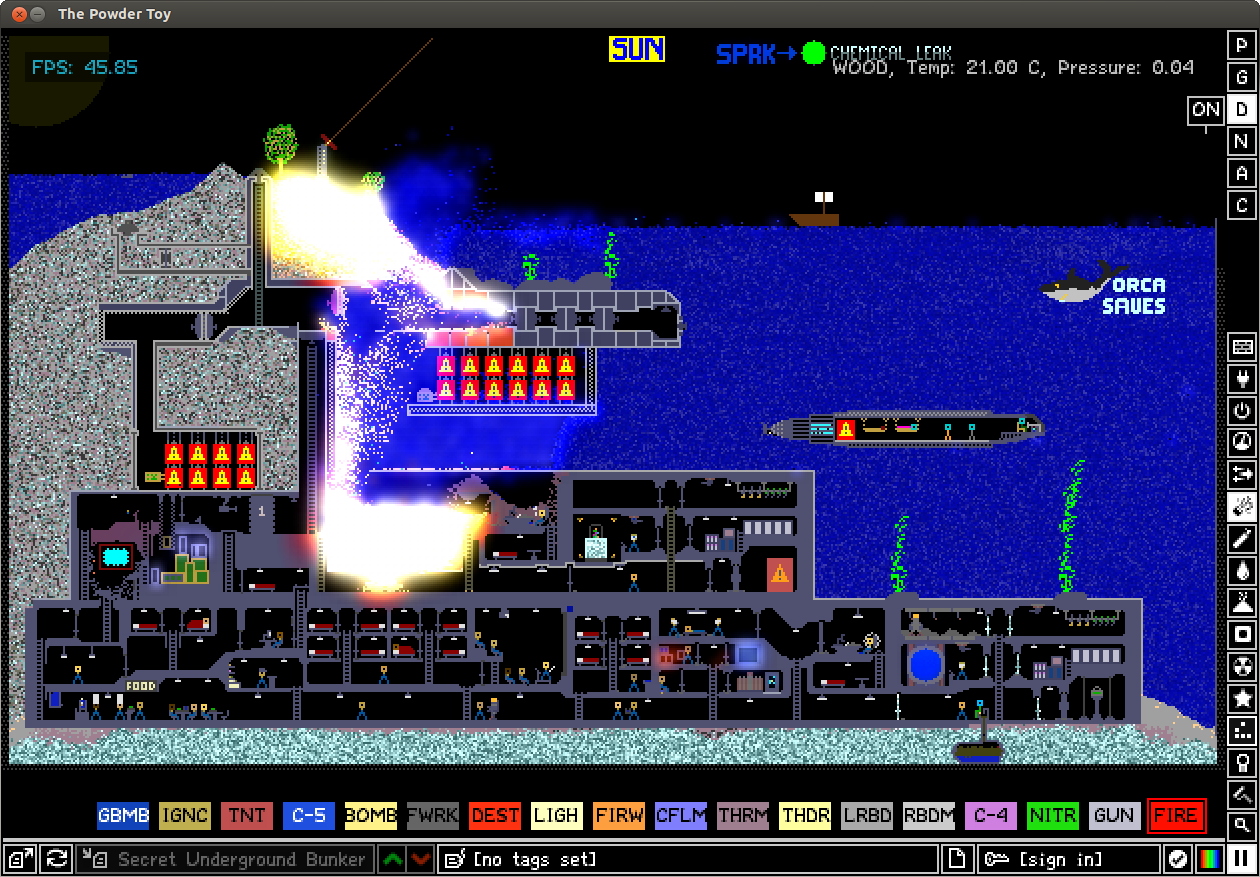
\includegraphics[width=\linewidth]{powdertoy/powdertoy-bu5.png}
\end{center}
Aber ein Teil des Meerwassers wird in die Luft geschleudert und die Stahlwände im Bunker fangen an rot zu glühen.
\begin{center}
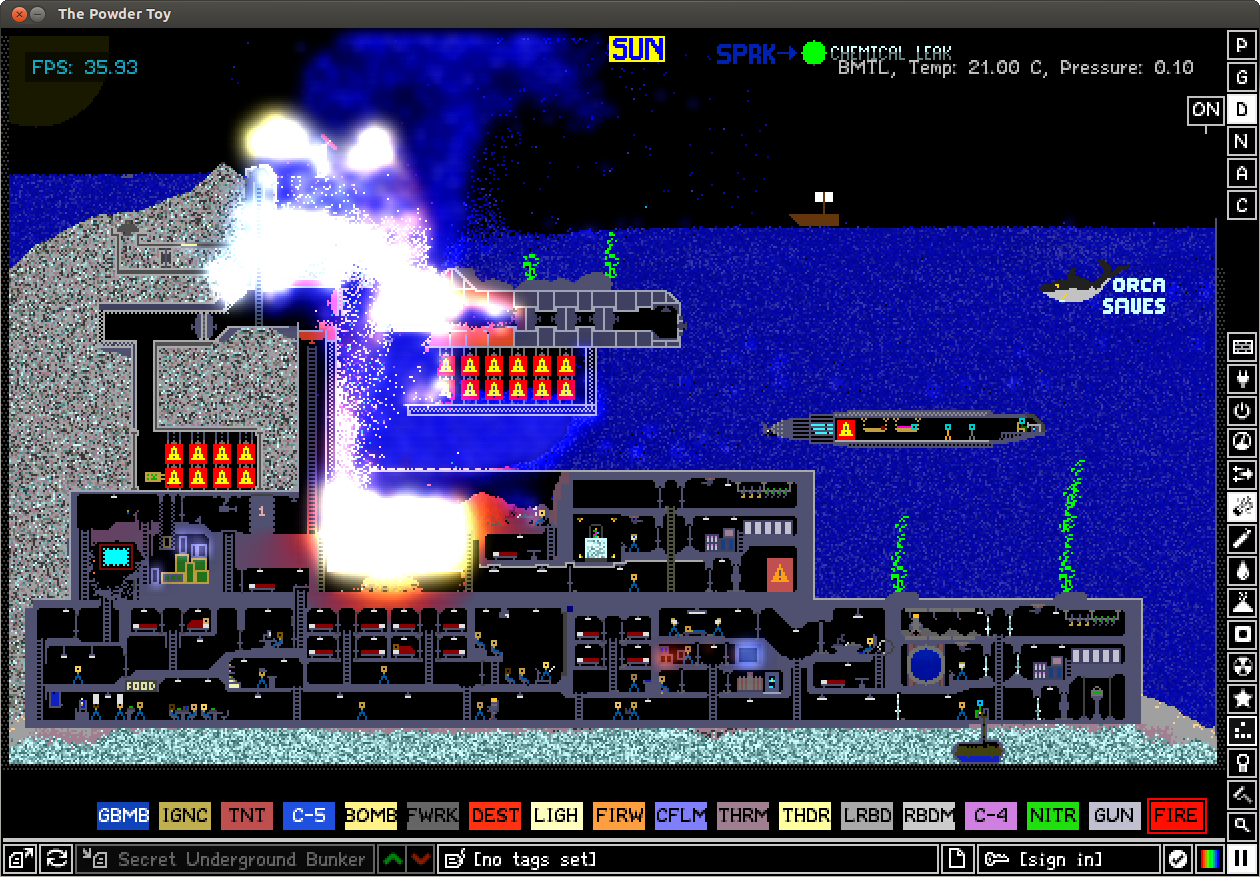
\includegraphics[width=\linewidth]{powdertoy/powdertoy-bu6.png}
\end{center}
Autsch, das waren die Giftfässer. Na, wenigstens sind sie nicht gerostet.
\begin{center}
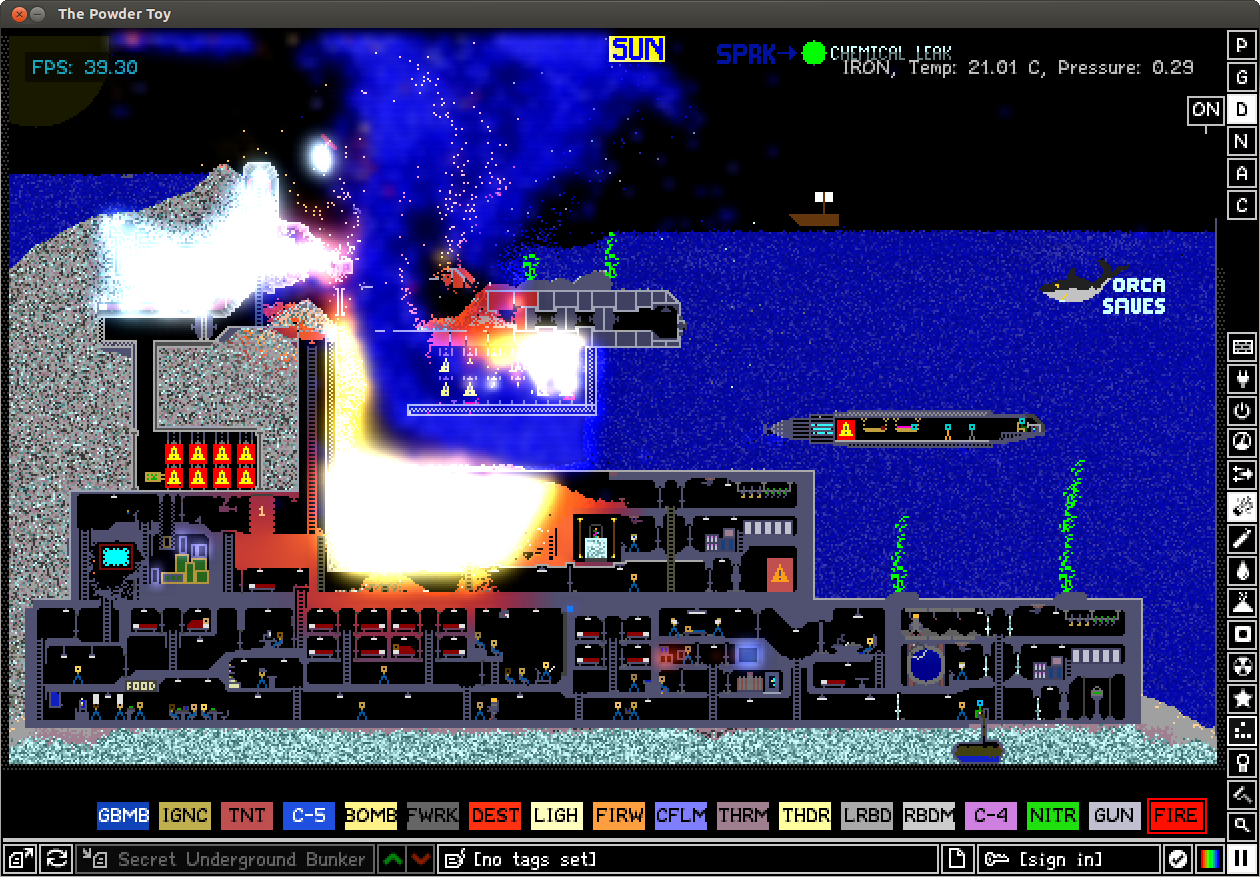
\includegraphics[width=\linewidth]{powdertoy/powdertoy-bu7.png}
\end{center}
Im Bunker wirds ganz schön heiss...
\begin{center}
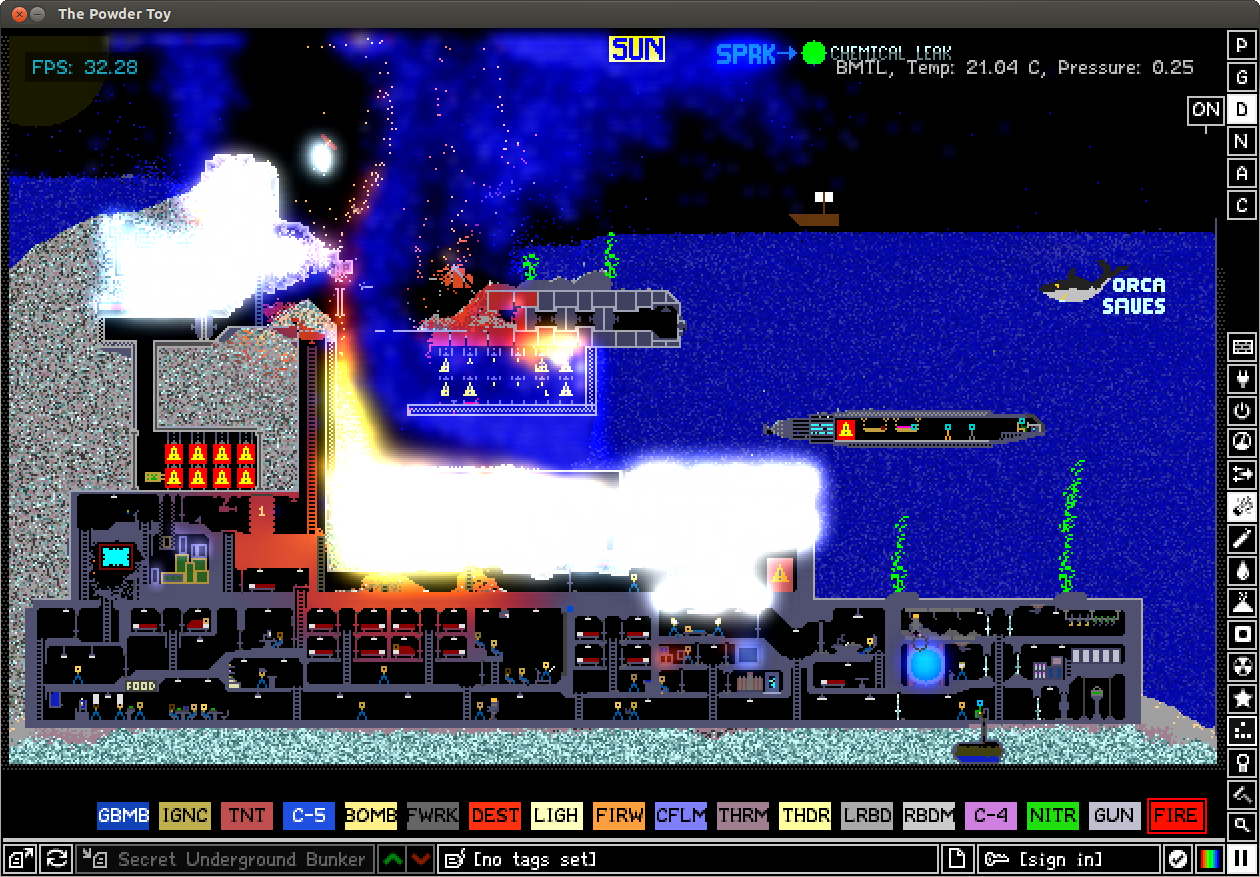
\includegraphics[width=\linewidth]{powdertoy/powdertoy-bu8.png}
\end{center}
Und das (dekorative, nicht-brennbare) Segelbot verliert durch die Verdampfung das Wasser unter dem Bug. Das U-Boot zeigt sich hingegen unbeeindruckt:
\begin{center}
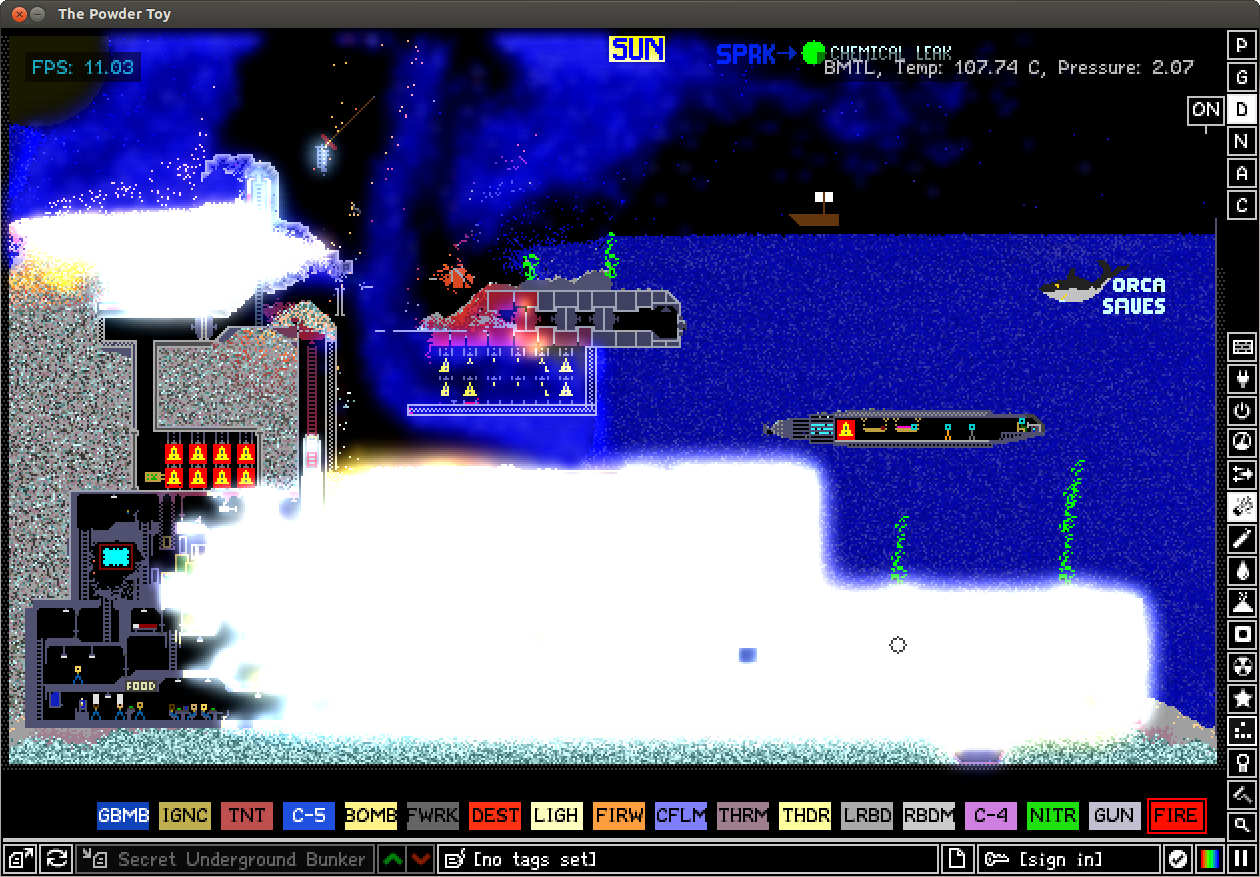
\includegraphics[width=\linewidth]{powdertoy/powdertoy-bu9.png}
\end{center}
Spät aber doch vertreibt die Hitze das verbliebene Wasser aus dem (ehemaligem) Giftfass-Raum wo es der thermische Aufwind nach oben treibt:
\begin{center}
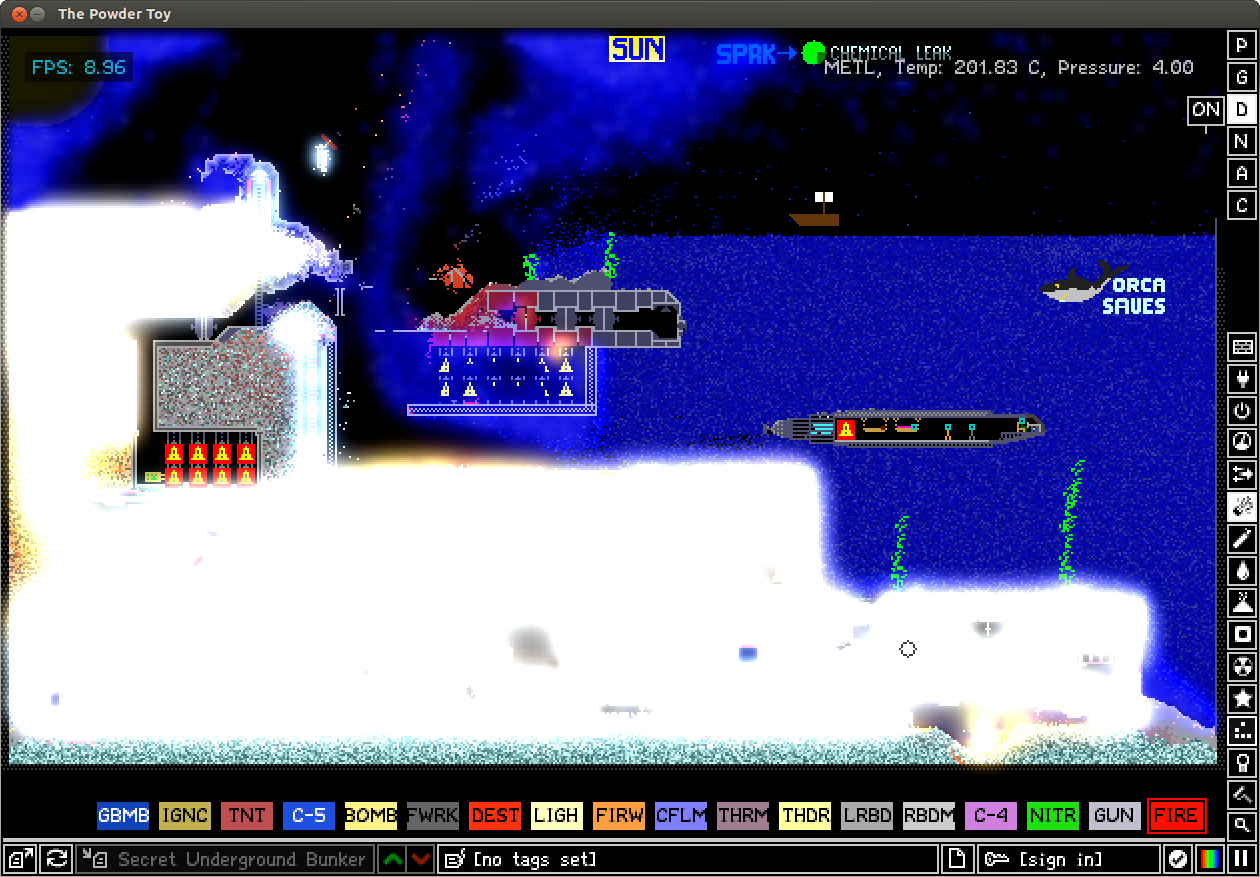
\includegraphics[width=\linewidth]{powdertoy/powdertoy-bu10.png}
\end{center}
Jetzt zerlegt es auch noch die letzten im Berg verbuddelten Giftfässer
\begin{center}
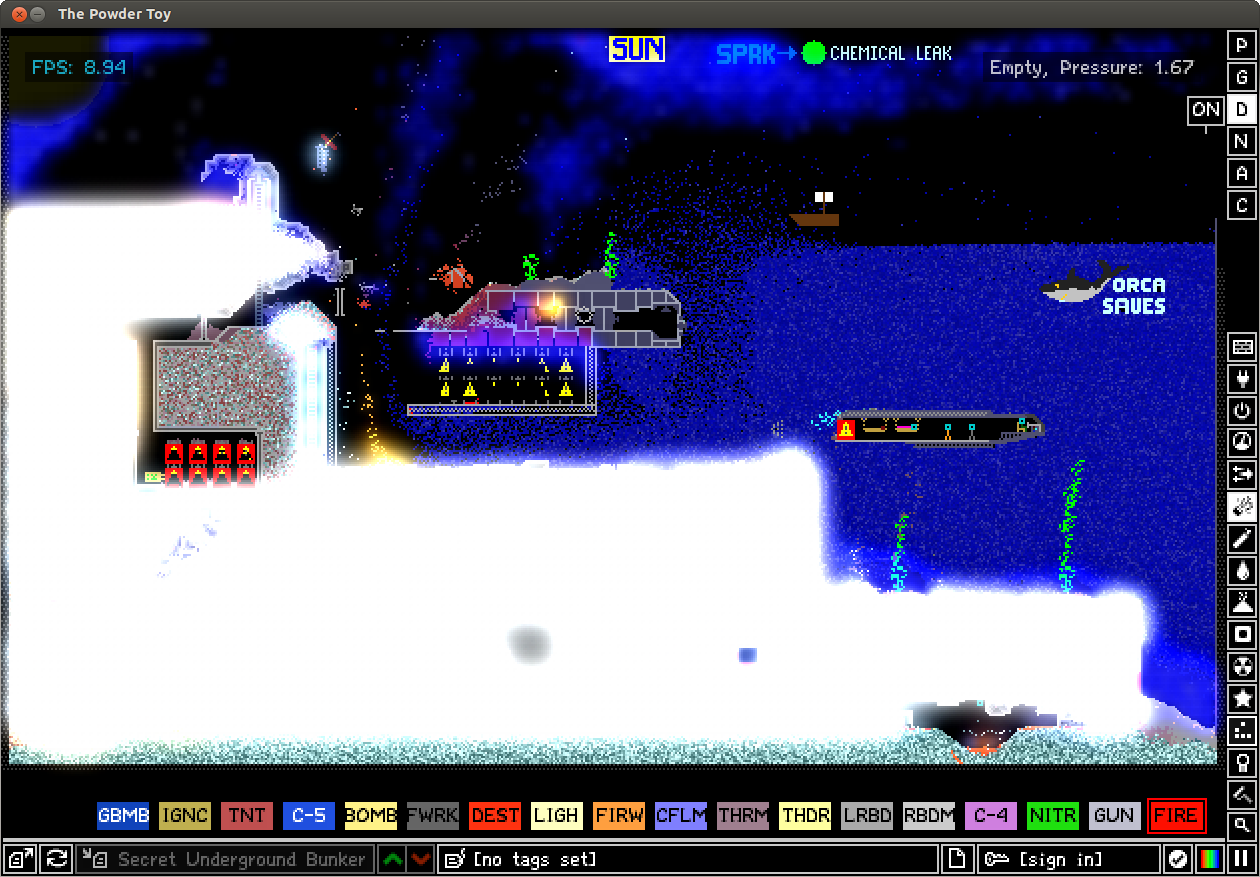
\includegraphics[width=\linewidth]{powdertoy/powdertoy-bu12.png}
\end{center}
Und auch das U-Boot kommt nicht ungeschoren davon:
\begin{center}
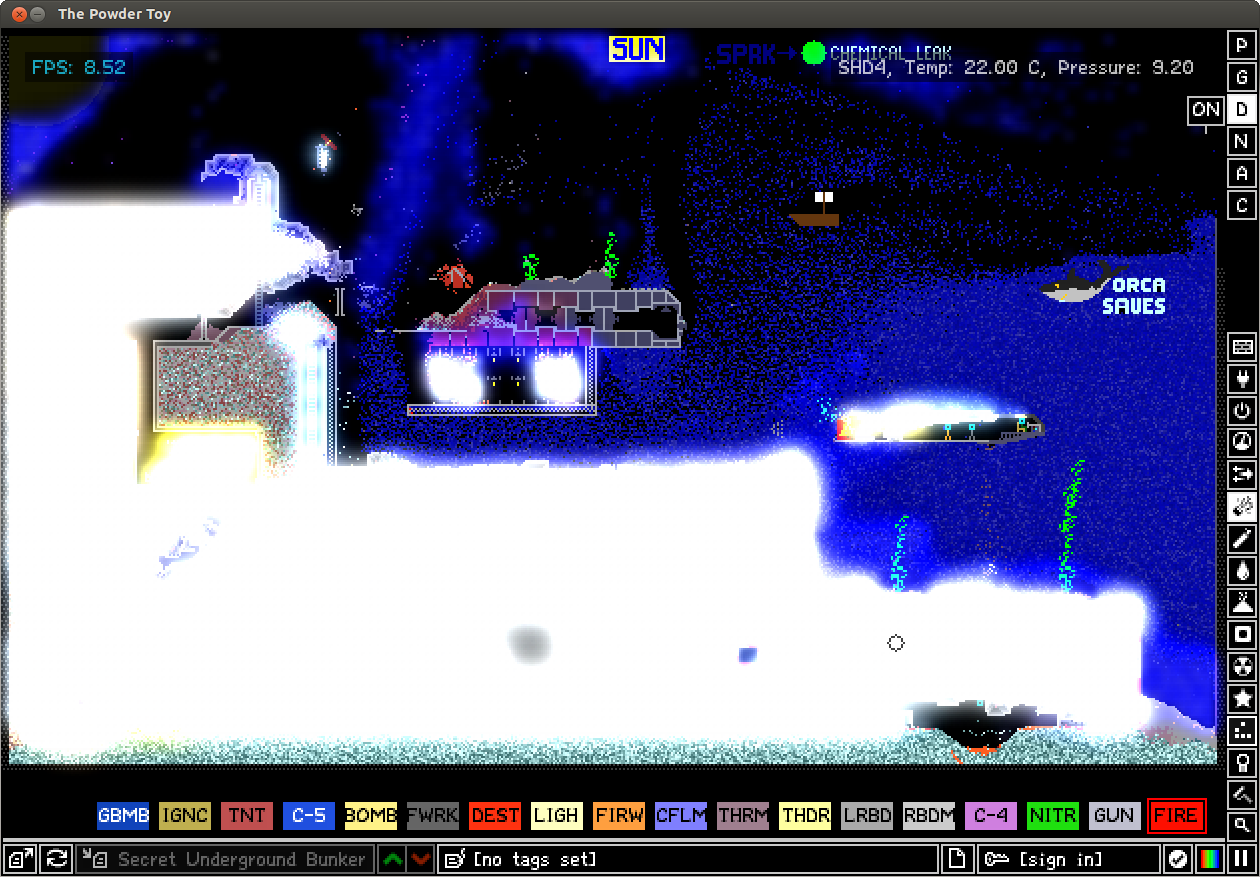
\includegraphics[width=\linewidth]{powdertoy/powdertoy-bu13.png}
\end{center}
Weder vom Bunker noch vom Meer bleibt viel übrig:
\begin{center}
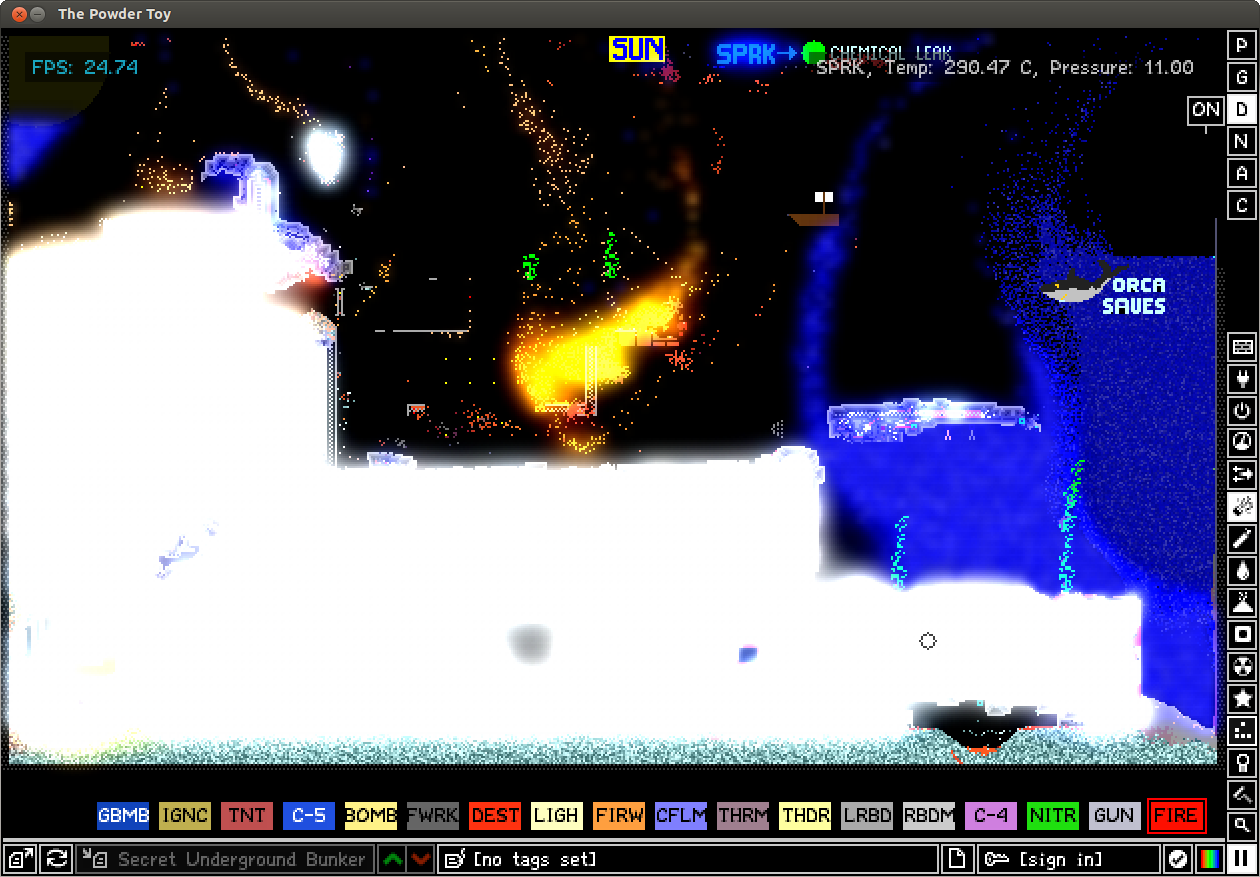
\includegraphics[width=\linewidth]{powdertoy/powdertoy-bu14.png}
\end{center}
Wie lange das Plasma im Bunker wohl brennt ?
\begin{center}
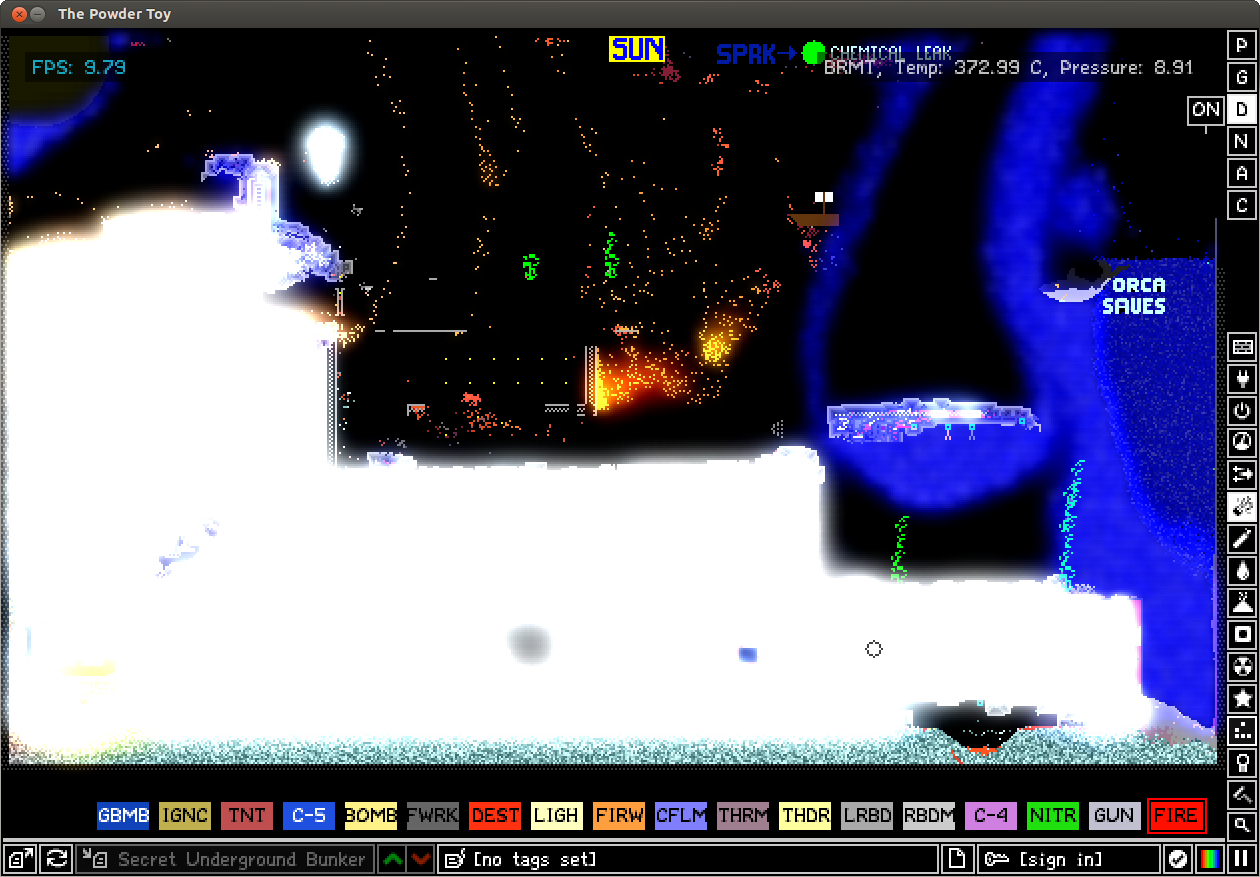
\includegraphics[width=\linewidth]{powdertoy/powdertoy-bu15.png}
\end{center}
Auch im Pause Modus kann man mittels Mauszeiger jederzeit Pixelgenau erfahren um welches Material es sich handelt und welchem Druck und welcher Temperatur er gerade ausgesetzt ist. 

\subsection*{Möglichkeiten}

Das Wiki der The Powder Game Homepage bietet ein Forum und ein FAQ sowie einige Tutorials. Man lernt wie man mittels Lua eigene Materialien mit eigenen Eigenschaften programmiert, man kann mittels The Powder Toy elektrische Schaltkreise und Logik-Schaltungen simulieren (umständlich) oder einfach schöne Pixelkunstwerke pinseln (und sie dann anzünden). Das Spiel bietet neben Elektrizität (leitende Materialien, Isolierungen etc.) auch Gravitation und Temperatur-Veränderer (im Echtzeitmodus) mit denen sich etwa Ventilatoren, Staubsauger oder schwarze Löcher simulieren lassen. Die Meisten Materialien interagieren mit anderen Materialien: Manche lassen nur Gas durch, manche nur Flüssigkeit, manche reagieren unterschiedlich auf Hitze oder Elektrizität. Besonders gefallen mir die Schaltflächen Game of Life mit denen man das scheinbar 'lebende' Organismen erschaffen kann (siehe \href{https://de.wikipedia.org/wiki/Conways_Spiel_des_Lebens}{\textit{Conways Game of Live}}) und die Specials, z.B. Materialien die Partikel verdoppeln (damit ist ein endloser Wasserfall möglich) oder die kleinen, per Tastatur steuerbaren 'Stickmen' und die sie jagenden 'Fighter'. 

\subsection*{Fachbegriffe:}

~~~\textbf{GPL Lizenz [2]}: garantiert die vier Grundfreiheiten 'to use, to stuy, to modify and to share'. \\ 

\textbf{Sourcecode} oder Quellcode sind die Programmzeilen aus denen ein Computerprogramm besteht. The Powder Toy ist in C++ geschrieben, für kleinere Veränderungen (z.B. ein neues Material hinzufügen) reichen aber Kenntnisse der relative leicht zu lernenden Programmiersprache \href{https://de.wikipedia.org/wiki/Lua}{\textit{Lua}}.

\textbf{komilieren, to compile} bedeutet ein Programm zu übersetzten, gemeint ist aus den Programmzeilen ein ausführbares Programm (binary) machen, mit Hilfe eines Compilers. 

\subsection*{Download, Feedback:}
\textbf{R.I.S.-Journal}, Ausgabe 001: \\
\href{http://spielend-programmieren.at/de:ris:001}{spielend-programmieren.at/de:ris:001}\\
\textbf{Download} Ordner, verschiedene Formate:\\
\href{http://spielend-programmieren.at/risjournal/001/powdertoy}{\texttt{spielend-programmieren.at/risjournal/001/powdertoy}} \\
\textbf{Feedback} \Letter\ \texttt{horst.jens@spielend-programmieren.at} \\


\subsection*{Lizenz, Quellen:}
\begin{wrapfigure}{l}{2.0cm}

\includegraphics[width=2cm]{powdertoy/ccbysa88x31.png}
\end{wrapfigure}
Dieses Material steht unter der Creative-Commons-Lizenz Namensnennung - Weitergabe unter gleichen Bedingungen 4.0 International. Um eine Kopie dieser Lizenz zu sehen, besuchen Sie \url{http://creativecommons.org/licenses/by-sa/4.0/deed.de}.

\textbf{Quellen:} \\
{[}1{]} \href{http://powdertoy.co.uk/}{powdertoy.co.uk/} \\
{[}2{]} \href{http://www.gnu.org/philosophy/free-sw.de.html}{gnu.org/philosophy/free-sw.de.html} \\
{[}3{]} \href{http://spielend-programmieren.at}{spielend-programmieren.at} \\
{[}4{]} \href{http://goo.gl/LK4z01}{goo.gl/LK4z01} \\
